\documentclass{article}
\usepackage{graphicx}
\usepackage{amsmath}
\usepackage{xcolor}
\usepackage{tikz}
\usetikzlibrary{automata, positioning, arrows}




\begin{document}

\title{Automi, Calcolabilità e Complessità}
\author{Alessandro Savioli}
\date{Ottobre 2024}

\maketitle

\tableofcontents

\newpage

\section{Prefazione}

La teoria della computazione inizia con una semplice domanda, \textbf{"Cos'è un
computer?}, al giorno d'oggi chiunque potrebbe rispondere, ma i computer reali
sono piuttosto complessi per permetterci di sviluppare una teoria matematica
direttamente su di essi, per questo serve avvalersi di un "Computer Ideale",
chiamato \textcolor{red}{Modello Di Computazione}.

Come per ogni modello scientifico un modello di computazione può essere accurato
in alcuni aspetti ma non rispetto ad altri, per questo lungo il corso ne useremo
diversi, a seconda delle caratteristiche su cui ci vogliamo soffermare.

Iniziamo quindi con il modello più semplice, chiamato \textbf{Macchina a stati
finiti} oppure \textbf{Automa finito}.

\section{Automi Finiti}
Gli automi finiti sono un buon modello per computer con una quantità
estremamente limitata di memoria. Essi sono alla base di vari dispositivi
elettromeccanici. 

Il sistema di controllo per una porta automatica è un esempio di tale
dispositivo, esse si aprono quando il sistema di controllo avverte che una
persona si sta avvicinando. 

Questo tipo di porte, che si possono trovare spesso alle entrate/uscite dei
supermercati, ha un sensore davanti per rilevare la presenza di una persona che
sta per attraversare la soglia, mentre un altro sensore è collocato dall'altro
lato in modo che il sistema possa mantenere la porta aperta finchè la persona
possa attraversarla in tranquillità. 

Possiamo raffigurare la disposizione in questo modo: 

\begin{center}
    \textcolor{red}{Ricordati di mettere l'immagine (porta supermercato)}
\end{center}

Questo sistema di controllo può essere in 2 diversi stati, \textbf{OPEN} o
\textbf{CLOSED}, che rappresentano la condizione corrispondente alla porta,
mentre possono esserci quattro condizioni di input: \textbf{"FRONT", "REAR",
"BOTH", "NEITHER"}

\begin{center}    
    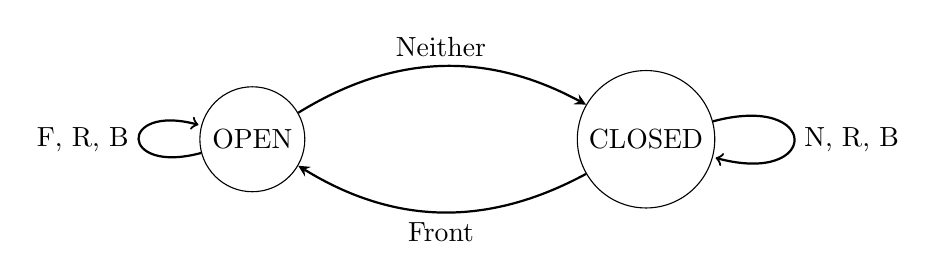
\begin{tikzpicture} [node distance = 5cm, on grid, auto]
        \node (OPEN)[state, left] {OPEN}; \node (CLOSED)[state, right = of OPEN]
        {CLOSED};
        \path [-stealth, thick]
        (OPEN) edge [loop left]  node {F, R, B}() (CLOSED) edge [loop right]
        node {N, R, B}() (OPEN) edge [bend left] node {Neither}   (CLOSED)
        (CLOSED) edge [bend left] node {Front}   (OPEN);
    \end{tikzpicture}
\end{center} 

Esaminiamo ora gli automi finiti da una prospettiva matematica. Svilupperemo una
definizione precisa di automa finito, una terminologia per descriverli e usarli,
e risultati teorici per descrivere il loro potere e i loro limiti.

\begin{center}
    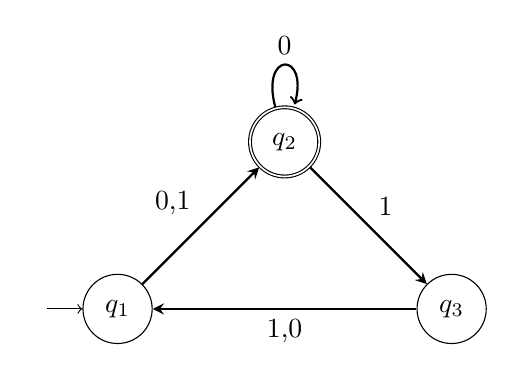
\begin{tikzpicture} [node distance = 3cm, on grid, auto]

        \node (q0) [state, initial, initial text = {}] {$q_1$}; \node (q1)
        [state, accepting, above right = of q0] {$q_2$}; \node (q2) [state,
        below right = of q1] {$q_3$};
        
        \path [-stealth, thick]
            (q0) edge node {0,1}   (q1) (q1) edge node {1}   (q2) (q1) edge
            [loop above]  node {0}() (q2) edge node {1,0} (q0);
    \end{tikzpicture}
\end{center}

Questo tipo di schema viene chiamato \textbf{Diagramma di stato}, esso ha tre
stati, etichettati q1 q2 e q3, lo \textbf{Stato iniziale} q1 è indicato
dall'arco entrante in esso e non uscente da un altro stato. Lo \textbf{Stato
accettante} q2 è indicato da un doppio cerchio. Gli archi che vanno da uno stato
all'altro vengono detti \textbf{Transizioni}.

Quando questo automa riceve una stringa in input come 1100, esso la elabora e
produce un output, che può essere \textbf{Accetta} o \textbf{Rifiuta}, a seconda
se alla fine della lettura dell'input, la macchina si trovi o meno in uno stato
accettante, considerando per ora solo questo tipo di output sì/no.

\subsection{Definizione Formale di Automa Finito}

\textcolor{red}{Definizione}
Un automa finito è una quintupla (Q, $\Sigma$, $\delta$, $q_0$, F), dove
\begin{enumerate}
    \item Q è un insieme finito chiamato insieme degli \textbf{stati}
    \item $\Sigma$ è un insieme finito chiamato \textbf{alfabeto}
    \item $\delta$ : Q x $\Sigma$ $\rightarrow$ Q è la \textbf{funzione di
    transizione}
    \item $q_0$ $\in$ Q è lo \textbf{stato iniziale}
    \item F $\subseteq$ Q è l'\textbf{insieme degli stati accettanti}
\end{enumerate}

Successivamente diremo che se A è l'insieme di tutte le stringe che una macchina
M accetta, allora chiameremo A il \textbf{Linguaggio della macchina M} e
scriveremo

\begin{center}
    \textbf{L(M) = A}
\end{center}

\subsection{Definizione Formale di Computazione}

\textcolor{red}{Definizione}
Sia M = (Q, $\Sigma$, $\delta$, $q_0$, F) un automa finito e sia w =
$w_1w_2...w_n$ una stringa dove ogni $w_i$ è un elemento dell'alfabeto $\Sigma$.

allora M \textbf{accetta} w se esiste una sequenza di stati $r_0, r_1, ..., r_n$
in Q con tre condizioni:

\begin{enumerate}
    \item $r_0 = q_0$
    \item $\delta (r_i, w_i+1) = r_i+1$, per i = 0, ..., n-1
    \item $r_n \in F$
\end{enumerate}

\textcolor{red}{Definizione}
Un linguaggio viene chiamato \textbf{Linguaggio Regolare} se esiste un automa
finito che lo riconosce

\subsection{Le Operazioni Regolari}
In aritmetica, gli oggetti di base sono i numeri e gli strumenti sono le
operazioni per trattarli, come + e $\times$. Nella teoria della computazione,
gli oggetti sono i linguaggi e gli strumenti includono operazioni
specificatamente progettate per trattarli. Definiamo tre operazioni sui
linguaggi, chiamate \textbf{Operazioni Regolari}, e le usiamo per studiare le
proprietà dei linguaggi regolari.

\textcolor{red}{Definizione}
Siano A e B linguaggi. Definiamo le operazioni regolari \textbf{Unione,
Concatenazione e Star} come segue:
\begin{itemize}
    \item \textbf{Unione}: A $\cup$ B = \{x $\mid$ x $\in$ A o x $\in$ B\}
    \item \textbf{Concatenazione} : A $\circ$ B = \{xy $\mid$ x $\in$ A e y
    $\in$ B\}
    \item \textbf{Star} $A^*$ = \{$x_1x_2...x_k$ $\mid$ k $\geq$ 0 e ogni $x_i
    \in A$\}
\end{itemize}

\textcolor{green! 50! black}{Teorema}

La classe dei linguaggi regolari (REG) è chiusa rispetto all'operazione di
unione e concatenazione.

In altre parole,
\begin{enumerate}
    \item Se $A_1 e A_2$ sono linguaggi regolari, anche $A_1 \cup A_2$ lo sarà
    \item Se $A_1 e A_2$ sono linguaggi regolari, anche $A_1 \circ A_2$ lo sarà
\end{enumerate}

\subsection{Non Determinismo}

Il non determinismo è un concetto utile che ha avuto un grande impatto sulla
teoria della computazione.

Finora ogni passo della computazione seguiva univocamente dal passo precedente,
facendoci parlare così di macchina \textbf{deterministica}.

In una macchina \textbf{non deterministica}, invece, possono esistere diverse
scelte per lo stato successivo. Il non determinismo è una generalizzazione del
determinismo, quindi \textsc{ogni automa finito deterministico è automaticamente
un automa finito non deterministico}.

In un DFA le etichette sugli archi di transizione sono simboli dell'alfabeto,
mentre in un NFA si possono avere archi etichettati con simboli dell'alfabeto e
un nuovo tipo di arco, etichettato con "$\varepsilon$", chiamato epsilon-arco.

\noindent \textcolor{red}{Come computa un NFA?}

Supponiamo di eseguire un NFA su una stringa di input e di giungere in uno stato
con più modi di procedere, dopo aver letto il simbolo in input, la macchina si
divide in \textbf{più copie di sé stessa e segue tutte le possibilità in
parallelo}, se ci sono scelte successive, la macchina si divide di nuovo. Se
invece ci imbattiamo in un epsilon-arco, accade qualcosa di simile, senza
leggere nessun input la macchina si divide in più copie, una che segue ciascun
arco uscente etichettato con $\varepsilon$ e una che resta nelllo stato
corrente.

\textcolor{red}{Definizione formale di automa finito non deterministico}

Un DFA e un NFA hanno una definizione formale molto simile, essi infatti
differiscono solo nella funzione di transizione, in un DFA quest'ultima prende
uno stato e un simbolo in input e produce lo stato successivo, mentre in un NFA
prende uno stato e un simbolo in input (o $\varepsilon$) e produce l'insieme dei
possibili stati successivi.

Un automa finito non deterministico è una quintupla (Q, $\Sigma$, $\delta$,
$q_0$, F), dove
\begin{enumerate}
    \item Q è un insieme finito chiamato insieme degli \textbf{stati}
    \item $\Sigma$ è un insieme finito chiamato \textbf{alfabeto}
    \item $\delta$ : Q x $\Sigma_\varepsilon$ $\rightarrow$ $\mathcal{P}(Q)$ è
    la \textbf{funzione di transizione}
    \item $q_0$ $\in$ Q è lo \textbf{stato iniziale}
    \item F $\subseteq$ Q è l'\textbf{insieme degli stati accettanti}
\end{enumerate}

\textcolor{green! 50! black}{teorema}
Per ogni automa finito non deterministico esiste un automa finito deterministico
equivalente (due macchine sono \textbf{equivalenti} se esse riconoscono lo
stesso linguaggio).

\subsection{Espressioni Regolari}

In aritmetica possiamo usare i simboli + e $\times$ per costruire espressioni
del tipo:

\begin{center}
    (5 + 3) $\times$ 4
\end{center}

Analogamente, possiamo usare le nostre operazioni regolari per costruire
espressioni che descrivono linguaggi, chiamate \textbf{Espressioni Regolari},
come:

\begin{center}
    (0 $\cup$ 1) $0^*$
\end{center}

Il valore dell'espressione aritmetica scritta sopra è 32, mentre il valore
dell'es-pressione regolare è un linguaggio, in questo caso un linguaggio che
consiste in \textbf{tutte le stringhe che iniziano con uno 0 o un 1 seguito da
qualsiasi numero di simboli uguali a 0}.

\textcolor{red}{Definizione Formale di Espressione Regolare}

\noindent Diciamo che R è un espressione regolare se è:
\begin{enumerate}
    \item a per qualche a nell'alfabeto $\Sigma$;
    \item $\varepsilon$;
    \item $\emptyset$;
    \item ($R_1 \cup R_2$), dove $R_1$ ed $R_2$ sono espressioni regolari;
    \item ($R_1 \circ R_2$), dove $R_1$ ed $R_2$ sono espressioni regolari;
    \item ($R_1^*$), dove $R_1$ è un'espressione regolare.
\end{enumerate}

\textcolor{orange}{Osservazione} Non bisogna confondere le espressioni regolari
$\varepsilon$ e $\emptyset$, in quanto la prima rappresenta il linguaggio che
contiene una sola stringa, ovvero la stringa vuota, mentre la seconda
rappresenta il linguaggio che non contiene nessuna stringa.

\noindent L'ordine in una espressione regolare risulta essere il seguente:
\begin{center}
    Star, Concatenazione, Unione
\end{center}

\begin{center}
    \textcolor{red}{Teorema}
    
    \textbf{Un linguaggio è regolare se e solo se qualche espressione regolare lo descrive}
\end{center}

\noindent Questo teorema deve essere dimostrato in entrambe le direzioni, quindi
enunciamo ogni direzione in un lemma separato.

\begin{center}
    \textcolor{red}{Lemma}

    \textbf{Se un linguaggio è descritto da un'espressione regolare, allora esso è regolare}
\end{center}

\textcolor{blue}{Dimostrazione $\rightarrow$}

Supponiamo di avere un'espressione regolare R che descrive un linguaggio A.
Mostriamo come trasformare R in un NFA che riconosce A, in quanto se un NFA
riconosce A allora A è regolare.

Per farlo, consideriamo i 6 casi nella definizione di espressione regolare.

\begin{enumerate}
    \item R = a per qualche a $\in$ $\Sigma$. Allora L(R) = $\{a\}$ e il
    seguente NFA riconosce L(R).

\begin{center}
    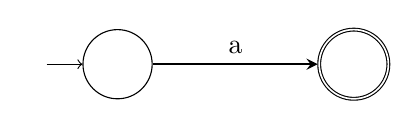
\begin{tikzpicture} [node distance = 3cm, on grid, auto]

        \node (q0) [state, initial, initial text = {}] {}; \node (q1) [state,
        accepting, right = of q0] {};
        
        \path [-stealth, thick]
            (q0) edge node {a}   (q1);
    \end{tikzpicture}
\end{center}

    Formalmente, N = (\{$q_1$, $q_2$\}, $\Sigma$, $\delta$, $q_1$, \{$q_2$\})

    \item R = $\varepsilon$. Allora L(R) = \{$\varepsilon$\} e il seguente NFA
    riconosce L(R).

\begin{center}
    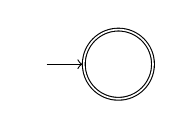
\begin{tikzpicture} [node distance = 3cm, on grid, auto]

        \node (q0) [state, initial, initial text = {}, accepting] {};

    \end{tikzpicture}
\end{center}

    Formalmente, N = (\{$q_1$\}, $\Sigma$, $\delta$, $q_1$, \{$q_1$\})

    \item R = $\emptyset$. Allora R = \{$\emptyset$\}, e il seguente NFA
    riconosce L(R).

\begin{center}
    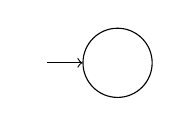
\begin{tikzpicture} [node distance = 3cm, on grid, auto]

        \node (q0) [state, initial, initial text = {}] {};

    \end{tikzpicture}
\end{center}

    Formalmente, N = (\{$q$\}, $\Sigma$, $\delta$, $q$, \{$\emptyset$\})

    \item R = $R_1 \cup R_2$.
    \item R = $R_1 \circ R_2$.
    \item R = $R^*_1$.
    
\end{enumerate}    

    Per gli ultimi tre casi, sappiamo che la classe dei linguaggi regolari è
    chiusa rispetto alle operazioni regolari, quindi non dovremo far altro che
    costruire l'NFA a partire da R visti nei primi 3 punti.

\begin{center}
    \textcolor{red}{Lemma}

    \textbf{Se un linguaggio è regolare, allora è descritto da un'espressione regolare.}
\end{center}

\textcolor{blue}{Dimostrazione $\leftarrow$}

Dobbiamo dimostrare che se un linguaggio A è regolare, allora un'espres-sione
regolare lo descrive. Poichè A è regolare, esso è accettato da un DFA.
Descriviamo quindi una procedura che permette di trasformare i DFA in
espressioni regolari equivalenti.

Dividiamo questa procedura in 2 parti, usando un nuovo tipo di automa finito
chiamato \textbf{Automa Finito non Deterministico Generalizzato} GNFA.

Prima mostriamo come trasformare un DFA in un GNFA e poi come trasformare un
GNFA in un'espresione regolare. 

Un GNFA legge blocchi di simboli dall'input, non necessariamente solo un simbolo
alla volta come in un comune NFA. Per comodità, richiediamo che ogni GNFA abbia
sempre una forma speciale che soddisfi le seguenti condizioni:

\begin{enumerate}
    \item Lo stato iniziale ha archi di transizione uscenti verso un qualsiasi
    altro stato ma nessun arco entrante proveniente da altri stati.
    \item Esiste un solo stato accettante, ed esso ha archi entranti provenienti
    da un qualsiasi altro stato ma nessun arco uscente verso altri stati,
    inoltre, lo stato accettante è diverso dallo stato iniziale.
    \item Eccetto che per lo stato iniziale e lo stato accettante, un arco va da
    ogni stato ad ogni altro stato e anche da ogni stato in sé stesso.
\end{enumerate}

Possiamo facilmente trasformare un DFA in un GNFA aggiungendo semplicemente un
nuovo stato iniziale con un $\varepsilon$-arco che entra nel vecchio stato
iniziale e un nuovo stato accettante con $\varepsilon$-archi entranti
provenienti dai vecchi stati accettanti.

Se alcuni archi hanno più etichette, sostituiamo ognuno di essi con un solo arco
la cui etichetta è l'unione delle precedenti etichette. Infine, aggiungiamo
archi con etichetta $\emptyset$ tra stati che non hanno archi. 

Successivamente, mostriamo come trasformare un GNFA in un'espressione regolare.
Supponiamo che il GNFA abbia k stati. Allora, poiché un GNFA deve avere uno
stato iniziale ed uno finale distinti, sappiamo che k $\geq$ 2. 

Se k $>$ 2, costruiamo un GNFA equivalente con k - 1 stati. Questo passo può
essere svolto fino a quando il nostro GNFA avrà solo due stati, quindi stato
iniziale e stato accettante, e l'etichetta dell'arco di transizione che li
collega sarà proprio la nostra \textbf{Espressione Regolare}.

\begin{center}
    \textcolor{red}{MANCA FINE DIMOSTRAZIONE}    
\end{center}

\subsection{Linguaggi Non Regolari}
Possiamo dire con certezza se tutti i linguaggi sono regolari oppure no? Si, ad
esempio sappiamo che:

\begin{center}
    L = \{$0^n 1^n : n \geq 0$\}

    NON è un linguaggio regolare.
\end{center}

Possiamo facilmente vedere che in un DFA con numero di stati $=$ n, ricevendo un
input w con $|w| > n$, ci dovranno essere degli stati ripetuti.

\subsubsection{Pumping Lemma}
La nostra tecnica per provare se un linguaggio sia regolare o meno deriva da un
teorema sui linguaggi regolari, chiamato Pumping Lemma. Questo teorema afferma
che tutti i linguaggi regolari hanno una proprietà speciale.

La proprietà afferma che tutte le stringhe nel linguaggio possono essere
"replicate" se la loro lunghezza raggiunge almeno uno specifico valore, chiamato
\textbf{Lunghezza del Pumping}. Questo significa che ogni tale stringa contiene
una parte che può essere ripetuta un numero qualsiasi di volte ottenendo una
stringa che appartiene ancora al linguaggio.

\begin{center}
    \textcolor{red}{Teorema: Pumping Lemma}
\end{center}

Se A è un linguaggio regolare, allora esiste un numero p (la lunghezza del
pumping) tale che se s è una qualsiasi stringa in A di lunghezza almeno p,
allora s può essere scomposta in tre parti, s = xyz, che soddisfano le seguenti
condizioni:

\begin{enumerate}
    \item per ogni i $\geq$ 0, $xy^iz \in A$,
    \item $|y| > 0$,
    \item $|xy| \leq p$.
\end{enumerate}

\textcolor{blue}{Dimostrazione}

Sia M = (Q, $\Sigma$, $\delta$, $q_1$, F) un DFA che riconosce A e sia p il
numero di stati di M. 

Sia s = $s_1s_2...s_n$ un stringa in A di lunghezza n dove n $\geq$ p. Sia $r_1,
..., r_n+1$ la sequenza di stati attraversati da M mentre elabora s, quindi
$\delta(r_i,s_i) = r_i+1$ per i compreso tra 1 ed n. Questa sequenza ha
lunghezza n + 1, che è almeno p + 1. Due tra i primi p + 1 elementi nella
sequenza devono essere lo stesso stato, per il \textbf{principio della
piccionaia}. 

Chiamiamo il primo di questi $r_i$ e il secondo $r_j$. Poichè $r_j$ si presenta
tra le prime p + 1 posizioni in una sequenza che inizia in $r_1$, abbiamo j
$\leq$ p + 1. 

Ora sia x = $s_1...s_i-1$, y = $s_i...s_j-1$ e z = $s_j...s_n$.

Poichè x porta M da $r_1$ a $r_i$, y porta M da $r_i$ a $r_i$ e z porta M da
$r_i$ a $r_n+1$, che è uno stato accettante, M deve accettare $xy^iz$ per i
$\geq$ 0. Sappiamo che i $\neq$ j, perciò $|y| > 0$

e j $\leq$ p + 1, perciò $|xy| \leq p$. Quindi tutte le condizioni del pumping
lemma sono rispettate.

\section{Linguaggi Context-Free}

Presentiamo ora le \textbf{Grammatiche Context-Free}, un metodo più potente per
scrivere linguaggi. Queste grammatiche possono descrivere alcuni aspetti che
hanno una struttura ricorsiva, che le rende utili in una varietà di
applicazioni.

Un'importante applicazione delle grammatiche si trova nella specifica e nella
compilazione dei linguaggi di programmazione, infatti la maggior parte dei
compilatori e degli interpreti contiene una componente chiamata \textbf{Parser}
che estrae il significato di un programma prima di generare il codice compilato
o di eseguire il programma interpretato.

I linguaggi associati alle grammatiche context-free sono chiamati
\textbf{Linguaggi Context-Free}. La classe di questi linguaggi include tutti i
linguaggi regolari e molti ulteriori linguaggi.

In questo capitolo diamo una definizione delle grammatiche context-free e
studiamo le proprietà dei linguaggi context-free. Introduciamo anche gli
\textbf{Automi a Pila} (pushdown automata), una classe di macchine che
riconoscono i linguaggi enunciati poco fa.

\subsection{Grammatiche Context-Free}

Un esempio di grammatica context-free, che chiamiamo $G_1$, è il seguente:

\begin{center}
    A $\rightarrow$ 0A1

    A $\rightarrow$ B

    B $\rightarrow$ \#
    
\end{center}

Una grammatica consiste in una serie di regole di \textbf{sostituzione}, anche
chiamate \textbf{Produzioni}. Ogni regola appare come una linea nella
grammatica, costituita da un simbolo e una stringa separati da una freccia.

Il simbolo è chiamato \textbf{Variabile}, mentre la stringa consiste di
variabili e altri simboli chiamati \textbf{Terminali}.

Le variabili sono spesso rappresentate da lettere maiuscole, mentre i terminali
sono rappresentati da lettere minuscole, numeri o simboli speciali.

Una delle variabili è chiamata \textbf{Variabile Iniziale} (solitamente è quella
al lato sinistro della regola più in alto)

Una grammatica può essere usata per descrivere un linguaggio generando ogni
stringa del linguaggio nel seguente modo:

\begin{enumerate}
    \item Scrivi la variabile iniziale.
    \item Trova una variabile che è stata scritta e una regola che inizia con
    quella variabile, sostituisci la variabile scritta con il lato destro di
    quella regola.
    \item Ripeti il passo 2 fino a quando non ci sono più variabili.
\end{enumerate}

Una sequenza di sostituzioni per ottenere una stringa è chiamata \textbf{Deri-
\\ vazione}.

Tutte le stringhe generate in questo modo costituiscono il \textbf{Linguaggio
della Grammatica}.

Denoteremo con L($G_1$) il linguaggio della grammatica $G_1$, che risulta essere
\{$0^n$\#$1^n$ $|$ n $\geq$ 0\}. Ogni linguaggio che può essere generato da una
grammatica context-free è chiamato \textbf{Linguaggio Context-Free} (CFL).

--------------------------------------------------------------------------------------------------

\begin{center}
    \textcolor{red}{Definizione Formale di Grammatica Context-Free}
\end{center}

Una grammatica context-free è una quadrupla (V, $\Sigma$, R, S), dove

\begin{enumerate}
    \item \textbf{V} è un insieme finito di variabili,
    \item \textbf{$\Sigma$} è un insieme finito, disgiunto da V, i cui elementi
    sono chiamati terminali,
    \item \textbf{R} è un insieme finito di regole,
    \item \textbf{S} $\in$ V, ovvero la variabile iniziale.
\end{enumerate}

--------------------------------------------------------------------------------------------------

se u, v e w sono stringhe di variabili e terminali e A $\rightarrow$ w è una
regola della grammatica, diciamo che uAv \textbf{Produce} uwv, e lo denotiamo
come uAv $\rightarrow$ uwv. 

Diciamo invece che u \textbf{Deriva} da v, e lo denotiamo con u $\rightarrow^*$
v, se u = v o se esiste una sequenza $u_1,u_2,...,u_k$ con k $\geq$ 0 e

\begin{center}
    u $\rightarrow$ $u_1$ $\rightarrow$ $u_2$ $\rightarrow$ ... $\rightarrow$
    $u_k$ $\rightarrow$ v
\end{center}

Qualche volta una grammatica può generare la stessa stringa in più modi diversi.
Tale stringa avrà dunque diversi alberi sintattici e quindi diversi significati.
Questo risultato può essere indesiderabile per alcune applicazioni, come i
\textbf{linguaggi di programmazione}, che dovrebbero avere un'unica
interpretazione. 

Se una grammatica genera la stessa stringa in più modi diversi, diremo che la
stringa è derivata \textbf{ambiguamente} in quella grammatica. 

Se una grammatica genera alcune stringhe ambiguamente, diremo che la grammatica
è \textbf{ambigua}.

Formalizziamo quindi la nozione di ambiguità. Quando diciamo che una grammatica
genera ambiguamente una stringa, intendiamo che la stringa ha almeno due diversi
alberi sintattici, non due diverse derivazioni, in quanto quest'ultime possono
differire solo nell'ordine in cui esse sostituiscono le variabili ma non nella
loro struttura complessiva.

Per concentrarci sulla struttura, definiamo un tipo di derivazione che
sostituisce le variabili con un ordine stabilito: la \textbf{Derivazione a
Sinistra} (leftmost derivation), che ad ogni passo sostituisce la variabile più
a sinistra.

\subsection{Forma Normale di Chomsky}

Quando si lavora con le grammatiche context-free, è spesso conveniente averle in
forma semplificata. Una delle forme più semplici e utili si chiama forma normale
di Chomsky.

--------------------------------------------------------------------------------------------------

\begin{center}
    \textcolor{red}{Definizione}
\end{center}

Una grammatica context-free è in \textbf{forma normale di Chomsky} se ogni
regola è della forma

\begin{center}
    A $\rightarrow$ BC

    A $\rightarrow$ a
\end{center}

dove "a" è un terminale e "A, B, C" sono variabili qualsiasi, tranne che B e C
non possono essere la variabile iniziale.

Inoltre, permettiamo la regola S $\rightarrow$ $\varepsilon$, dove S è la
variabile iniziale.

--------------------------------------------------------------------------------------------------

\subsection{Automi a Pila}

In questa sezione introduciamo un nuovo tipo di modello computazionale, chiamato
\textbf{automa a pila} (pushdown automata). Questi automi sono come gli automi
finiti non deterministici ma hanno una componente in più, chiamata \textbf{pila}
(stack). La pila fornisce memoria aggiuntiva, che consente a tali automi di
riconoscere alcuni linguaggi non regolari.

Gli automi a pila sono computazionalmente equivalenti alle grammatiche
context-free.

La figura seguente è una rappresentazione schematica di un automa finito. Il
controllo rappresenta gli stati e la funzione di transizione, il nastro contiene
la stringa di input e la freccia rappresenta la testina sull'input, che indica
il successivo simbolo da leggere.

\begin{center}
    
\tikzset{every picture/.style={line width=0.75pt}} %set default line width to
0.75pt        

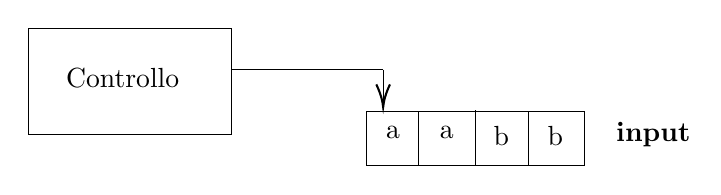
\begin{tikzpicture}[x=0.75pt,y=0.75pt,yscale=-1,xscale=1]
%uncomment if require: \path (0,300); %set diagram left start at 0, and has
%height of 300

%Shape: Rectangle [id:dp9416987304067759] 
\draw   (100,89) -- (198,89) -- (198,140) -- (100,140) -- cycle ;
%Shape: Rectangle [id:dp3803387153024198] 
\draw   (263,129) -- (368,129) -- (368,155) -- (263,155) -- cycle ;
%Straight Lines [id:da7053902512087236] 
\draw    (288,129) -- (288,155) ;
%Straight Lines [id:da5656119026072681] 
\draw    (341,129) -- (341,143) -- (341,155) ;
%Straight Lines [id:da6739796655004393] 
\draw    (315.5,128.5) -- (315.5,155.5) ;
%Straight Lines [id:da34292098732116805] 
\draw    (198,109) -- (271,109) ;
%Straight Lines [id:da9542933537032088] 
\draw    (271,109) -- (271,125) ; \draw [shift={(271,127)}, rotate = 270]
[color={rgb, 255:red, 0; green, 0; blue, 0 }  ][line width=0.75]
(10.93,-3.29) .. controls (6.95,-1.4) and (3.31,-0.3) .. (0,0) .. controls
(3.31,0.3) and (6.95,1.4) .. (10.93,3.29)   ;

% Text Node
\draw (117,107) node [anchor=north west][inner sep=0.75pt]   [align=left]
{Controllo};
% Text Node
\draw (271,135) node [anchor=north west][inner sep=0.75pt]   [align=left] {a};
% Text Node
\draw (297,135) node [anchor=north west][inner sep=0.75pt]   [align=left] {a};
% Text Node
\draw (323,135) node [anchor=north west][inner sep=0.75pt]   [align=left] {b};
% Text Node
\draw (349,135) node [anchor=north west][inner sep=0.75pt]   [align=left] {b};
% Text Node
\draw (382,133) node [anchor=north west][inner sep=0.75pt]   [align=left]
{\textbf{input}};


\end{tikzpicture}

\end{center}

Aggiungendo l'elemento pila, otteniamo una rappresentazione schematica di un
automa a pila, come mostrato nella figura seguente.

\begin{center}
    
\tikzset{every picture/.style={line width=0.75pt}}       

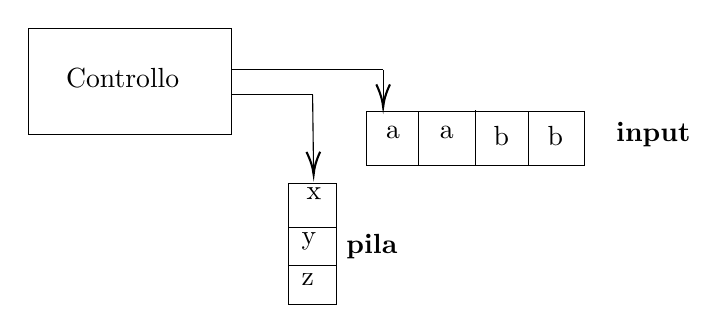
\begin{tikzpicture}[x=0.75pt,y=0.75pt,yscale=-1,xscale=1]
%uncomment if require: \path (0,300); %set diagram left start at 0, and has
%height of 300

%Shape: Rectangle [id:dp9416987304067759] 
\draw   (100,89) -- (198,89) -- (198,140) -- (100,140) -- cycle ;
%Shape: Rectangle [id:dp3803387153024198] 
\draw   (263,129) -- (368,129) -- (368,155) -- (263,155) -- cycle ;
%Straight Lines [id:da7053902512087236] 
\draw    (288,129) -- (288,155) ;
%Straight Lines [id:da5656119026072681] 
\draw    (341,129) -- (341,143) -- (341,155) ;
%Straight Lines [id:da6739796655004393] 
\draw    (315.5,128.5) -- (315.5,155.5) ;
%Straight Lines [id:da34292098732116805] 
\draw    (198,109) -- (271,109) ;
%Straight Lines [id:da9542933537032088] 
\draw    (271,109) -- (271,125) ; \draw [shift={(271,127)}, rotate = 270]
[color={rgb, 255:red, 0; green, 0; blue, 0 }  ][line width=0.75]
(10.93,-3.29) .. controls (6.95,-1.4) and (3.31,-0.3) .. (0,0) .. controls
(3.31,0.3) and (6.95,1.4) .. (10.93,3.29)   ;
%Straight Lines [id:da7703102214779298] 
\draw    (198,121) -- (237,121) ;
%Straight Lines [id:da18533887117997438] 
\draw    (237,121) -- (237.47,157.5) ; \draw [shift={(237.5,159.5)}, rotate =
269.26] [color={rgb, 255:red, 0; green, 0; blue, 0 }  ][line width=0.75]
(10.93,-3.29) .. controls (6.95,-1.4) and (3.31,-0.3) .. (0,0) .. controls
(3.31,0.3) and (6.95,1.4) .. (10.93,3.29)   ;
%Shape: Rectangle [id:dp0926240064959345] 
\draw   (225.5,164) -- (248.5,164) -- (248.5,222) -- (225.5,222) -- cycle ;
%Straight Lines [id:da13807730534670593] 
\draw    (225.5,185) -- (248.5,185) ;
%Straight Lines [id:da6591726489874976] 
\draw    (225.5,203.5) -- (248.5,203.5) ;

% Text Node
\draw (117,107) node [anchor=north west][inner sep=0.75pt]   [align=left]
{Controllo};
% Text Node
\draw (271,135) node [anchor=north west][inner sep=0.75pt]   [align=left] {a};
% Text Node
\draw (297,135) node [anchor=north west][inner sep=0.75pt]   [align=left] {a};
% Text Node
\draw (323,135) node [anchor=north west][inner sep=0.75pt]   [align=left] {b};
% Text Node
\draw (349,135) node [anchor=north west][inner sep=0.75pt]   [align=left] {b};
% Text Node
\draw (382,133) node [anchor=north west][inner sep=0.75pt]   [align=left]
{\textbf{input}};
% Text Node
\draw (232.98,164.43) node [anchor=north west][inner sep=0.75pt]  [rotate=-0.7]
[align=left] {x};
% Text Node
\draw (237.5,191.5) node   [align=left]
{\begin{minipage}[lt]{8.67pt}\setlength\topsep{0pt} y \end{minipage}};
% Text Node
\draw (237.5,210.25) node   [align=left]
{\begin{minipage}[lt]{8.67pt}\setlength\topsep{0pt} z \end{minipage}};
% Text Node
\draw (270.75,194) node   [align=left]
{\begin{minipage}[lt]{26.18pt}\setlength\topsep{0pt}
\textbf{pila}
\end{minipage}};


\end{tikzpicture}

\end{center}

Un automa a pila (PDA) può scrivere simboli nella pila e rileggerli in seguito.
Scrivere un simbolo "spinge giù" tutti gli altri simboli nella pila. In un
qualunque momento il simbolo sulla cima (top) della pila può essere letto e
rimosso, facendo risalire tutti gli altri simboli. 

L'operazione di scrittura sulla pila viene chiamata \textbf{push}, mentre quella
di eliminarne uno viene chiamata \textbf{pop}. Ricordiamo che ogni operazione,
sia di scrittura che di lettura, può essere effettuato solo sulla sommità.

La pila risulta essere molto importante perché permette di memorizzare una
quantità non limitata di informazioni. Ricordiamo che un automa finito non può
riconoscere il linguaggio \{$0^n1^n | $ n $\geq$ 0\} poiché non è in grado di
fare ciò che abbiamo appena enunciato.

--------------------------------------------------------------------------------------------------

\begin{center}
    \textcolor{red}{Definizione Formale di Automa a Pila}
\end{center}

un automa a pila è una sestupla (Q, $\Sigma$, $\Gamma$, $\delta$, $q_0$, F) dove
Q, $\Sigma$, $\Gamma$ ed F sono tutti insiemi finiti e:

\begin{enumerate}
    \item Q è l'insieme degli stati,
    \item $\Sigma$ è l'alfabeto dell'input,
    \item $\Gamma$ è l'alfabeto della pila,
    \item $\delta$ : Q $\times \Sigma_\varepsilon \times \Gamma_\varepsilon
    \rightarrow \mathcal{P} (Q \times \Gamma_\varepsilon)$ è la funzione di
    transizione,
    \item $q_0 \in Q$ è lo stato iniziale,
    \item F $\subseteq$ Q è l'insieme degli stati accettanti.
\end{enumerate}

--------------------------------------------------------------------------------------------------

\subsubsection{Equivalenza con le Grammatiche Context-Free}

In questa sezione mostriamo che grammatiche context-free e automi a pila sono
computazionalmente equivalenti, mostreremo come trasformare ogni grammatica
context-free in un automa a pila che riconosce lo stesso linguaggio e viceversa.

Ricordiamo che abbiamo definito un linguaggio context-free come un linguaggio
che può essere descritto con una grammatica context-free, quindi il nostro
obiettivo è il teorema seguente.

--------------------------------------------------------------------------------------------------

\begin{center}
    \textcolor{red}{Teorema}
\end{center}

Un linguaggio è context-free se e solo se esiste un automa a pila che lo
riconosce.

--------------------------------------------------------------------------------------------------

Andiamo a vedere dunque entrambi i lati del "se e solo se":

--------------------------------------------------------------------------------------------------

\begin{center}
    \textcolor{red}{Lemma $\rightarrow$}
\end{center}

Se è un linguaggio è context-free, allora esiste un automa a pila che lo
riconosce.

--------------------------------------------------------------------------------------------------

\textcolor{blue}{Idea e Dimostrazione $\rightarrow$}

\textbf{IDEA}. Sia A un CFL. Dalla definizione sappiamo che esiste una CFG, G,
che genera A. mostriamo come trasformare G in un PDA equivalente, che chiamiamo
P.

\textbf{DIMOSTRAZIONE}. Ora diamo i dettagli formali della costruzione
\\dell'automa a pila P = (Q, $\Sigma$, $\Gamma$, $\delta$, $q_start$, F). Per
rendere più chiara la costruzione, usiamo una notazione abbreviata per la
funzione di transizione. Questa notazione fornisce un modo per scrivere
un'intera stringa sulla pila in un passo della macchina.

questa notazione è (r, u) $\in$ $\delta$(q, a, s), denota che quando q è lo
stato in cui si trova l'automa, a è il prossimo simbolo di input ed s è il
simbolo sulla cima della pila, il PDA può leggere a ed eliminare s, poi inserire
la stringa u nella pila e passare allo stato r, la figura seguente mostra la
realizzazione.

\begin{center}
    \textbf{Versione Semplificata}

    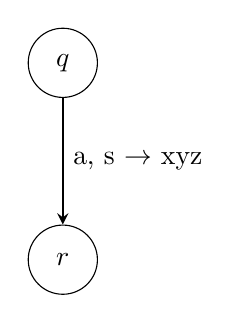
\begin{tikzpicture} [node distance = 2.5cm, on grid, auto]

        \node (q0) [state, initial text = {}] {$q$}; \node (q1) [state, below =
        of q0] {$r$};

        \path [-stealth, thick]
            (q0) edge node {a, s $\rightarrow$ xyz}  (q1);
            
    \end{tikzpicture}
\end{center}

\begin{center}
    \textbf{Versione Completa}

    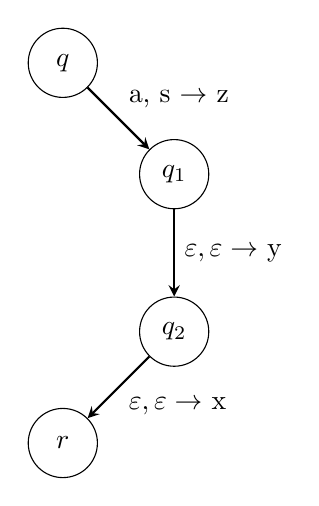
\begin{tikzpicture} [node distance = 2cm, on grid, auto]

        \node (q0) [state, initial text = {}] {$q$}; \node (q1) [state, below
        right = of q0] {$q_1$}; \node (q2) [state, below = of q1] {$q_2$}; \node
        (q3) [state, below left = of q2] {$r$};

        \path [-stealth, thick]
            (q0) edge node {a, s $\rightarrow$ z}  (q1) (q1) edge node
            {$\varepsilon , \varepsilon \rightarrow $ y}  (q2) (q2) edge node
            {$\varepsilon , \varepsilon \rightarrow $ x}  (q3);
            
    \end{tikzpicture}
\end{center}

Gli stati di P sono Q = \{$q_{start}, q_{loop}, q_{accept}$\} $\cup$ E, dove E è
l'insieme degli \textbf{stati intermedi} (come $q_1, q_2$ nel disegno sopra).

Il suo diagramma di stato è mostrato nella figura seguente.

\begin{center}
    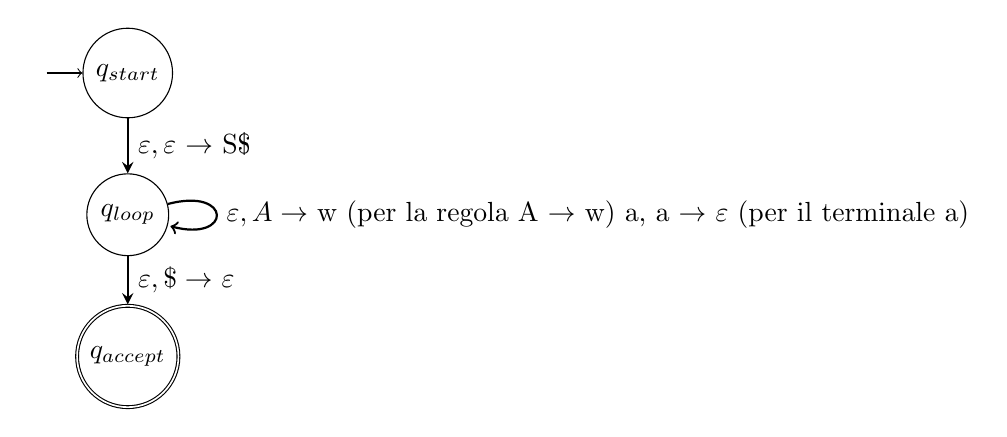
\begin{tikzpicture} [node distance = 1.8cm, on grid, auto]

        \node (q0) [state, initial, initial text = {}] {$q_{start}$}; \node (q1)
        [state, below = of q0] {$q_{loop}$}; \node (q2) [state, accepting, below
        = of q1] {$q_{accept}$};

        \path [-stealth, thick]
            (q0) edge node {$\varepsilon, \varepsilon$ $\rightarrow$ S\$}  (q1)
            (q1) edge [loop right] node {$\varepsilon , A \rightarrow $ w (per
            la regola A $\rightarrow$ w) a, a $\rightarrow$ $\varepsilon$ (per
            il terminale a)}   () (q1) edge node {$\varepsilon , \$ \rightarrow
            $ $\varepsilon$}  (q2);
            
    \end{tikzpicture}
\end{center}

Questo prova come un PDA può riconoscere un linguaggio context-free, passiamo
ora alla seconda implicazione.

--------------------------------------------------------------------------------------------------

\begin{center}
    \textcolor{red}{Lemma $\leftarrow$}
\end{center}

Se un linguaggio è riconosciuto da un automa a pila, allora esso è context-free.

--------------------------------------------------------------------------------------------------

\textcolor{blue}{Idea e Dimostrazione $\leftarrow$}

\textbf{IDEA}. Abbiamo un PDA P e vogliamo costruire una CFG G che genera tutte
le stringhe che P accetta. In altre parole, G dovrebbe generare una stringa se
quella stringa fa andare il PDA dal suo stato iniziale ad uno stato accettante.

Per raggiungere questo risultato, progettiamo una grammatica che fa un po' in
più. Per ciascuna coppia di stati p e q in P, la grammatica avrà una variabile
$A_{pq}$. Questa variabile genera tutte le stringhe che possono portare P da p
con pila vuota a q con pila vuota.

Innanzitutto, semplifichiamo il nostro compito modificando leggermente P per
munirlo delle seguenti 3 caratteristiche: 

\begin{enumerate}
    \item Ha un unico stato accettante, $q_{accept}$,
    \item Svuota la sua pila prima di accettare,
    \item Ciascuna transizione inserisce un simbolo sulla pila o ne elimina uno
    dalla pila, ma non può fare entrambe le cose.
\end{enumerate}

Per dare a P queste caratteristiche faremo come rappresentato nelle immagini
seguenti:

\begin{center}

--------------------------------------------------------------------------------------------------

    \textbf{Caratteristica 1}

--------------------------------------------------------------------------------------------------

    \textbf{Prima}

    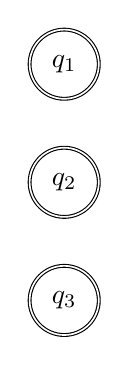
\begin{tikzpicture} [node distance = 1.5cm, on grid, auto]

        \node (q0) [state, accepting] {$q_1$}; \node (q1) [state, accepting,
        below = of q0] {$q_2$}; \node (q2) [state, accepting, below = of q1]
        {$q_3$};
            
    \end{tikzpicture}

    \textbf{Dopo}

    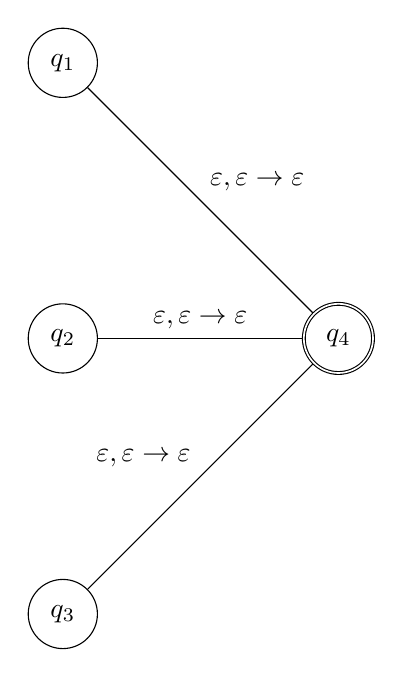
\begin{tikzpicture} [node distance = 3.5cm, on grid, auto]

        \node (q0) [state] {$q_1$}; \node (q1) [state, below = of q0] {$q_2$};
        \node (q2) [state, below = of q1] {$q_3$}; \node (q3) [state, accepting,
        right = of q1] {$q_4$};

        \draw
         (q0) edge node {$\varepsilon, \varepsilon \rightarrow \varepsilon$}
         (q3) (q1) edge node {$\varepsilon, \varepsilon \rightarrow
         \varepsilon$} (q3) (q2) edge node {$\varepsilon, \varepsilon
         \rightarrow \varepsilon$} (q3);
                    
    \end{tikzpicture}

--------------------------------------------------------------------------------------------------

    \textbf{Caratteristica 2}

--------------------------------------------------------------------------------------------------

    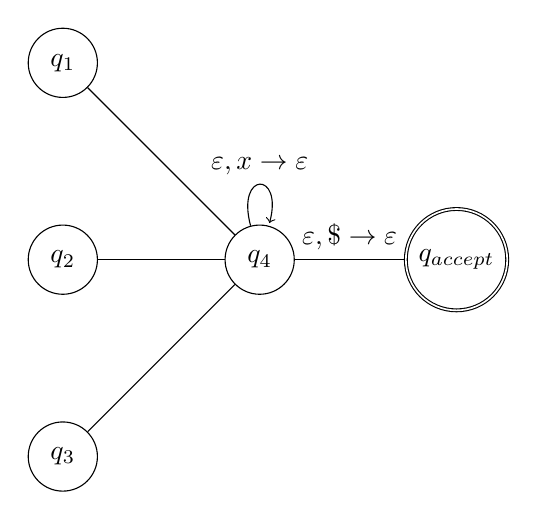
\begin{tikzpicture} [node distance = 2.5cm, on grid, auto]

        \node (q0) [state] {$q_1$}; \node (q1) [state, below = of q0] {$q_2$};
        \node (q2) [state, below = of q1] {$q_3$}; \node (q3) [state, right = of
        q1] {$q_4$}; \node (q4) [state, accepting, right = of q3]
        {$q_{accept}$};

        \draw
         (q0) edge node {} (q3) (q1) edge node {} (q3) (q2) edge node {} (q3)
         (q3) edge [loop above] node {$\varepsilon, x \rightarrow \varepsilon$}
         () (q3) edge node {$\varepsilon, \$ \rightarrow \varepsilon$} (q4);
                    
    \end{tikzpicture}

--------------------------------------------------------------------------------------------------

    \textbf{Caratteristica 3}

--------------------------------------------------------------------------------------------------    

    \textbf{Prima}

    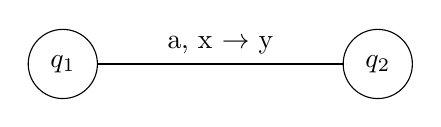
\begin{tikzpicture} [node distance = 4cm, on grid, auto]

        \node (q0) [state] {$q_1$}; \node (q1) [state, right = of q0] {$q_2$};

        \draw
        (q0) edge node {a, x $\rightarrow$ y} (q1);
            
    \end{tikzpicture}

    \textbf{Dopo}

    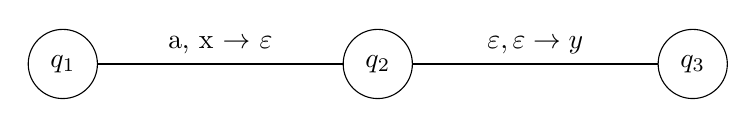
\begin{tikzpicture} [node distance = 4cm, on grid, auto]

        \node (q0) [state] {$q_1$}; \node (q1) [state, right = of q0] {$q_2$};
        \node (q2) [state, right = of q1] {$q_3$};

        \draw
        (q0) edge node {a, x $\rightarrow$ $\varepsilon$} (q1) (q1) edge node
        {$\varepsilon, \varepsilon \rightarrow y$} (q2);
            
    \end{tikzpicture}

\end{center}

Successivamente, per progettare G in modo tale che $A_{pq}$ generi tutte le
stringhe che portano P da p a q, iniziando e terminando con una pila vuota,
dobbiamo capire come P agisce su queste stringhe. Per ognuna di queste stringhe
x, la prima mossa di P su x deve essere un push, poiché P non può eliminare da
una pila vuota. Analogamente, l'ultima mossa di P sarà un pop perché alla fine
la pila deve essere vuota.

Durante la computazione di P su x si presentano due eventualità:

\begin{enumerate}
    \item il simbolo eliminato alla fine è il simbolo inserito all'inizio,
    quindi la pila non si è svuotata nel mezzo;
    \item il simbolo eliminato alla fine \textbf{non} è il simbolo inserito
    all'inizio, quindi la pila si è svuotata nel mezzo.
\end{enumerate}

Simuliamo la prima possibilità con la regola

\begin{center}
    $A_{pq} \rightarrow aA_{rs}b$
\end{center}

Dove a è l'input letto nella prima mossa, b è l'input letto nell'ultima mossa, r
è lo stato che segue p e s è lo stato che precede q.

Simuliamo la seconda possibilità con la regola

\begin{center}
    $A_{pq} \rightarrow A_{pr}A_{rq}$
\end{center}

Dove r è lo stato in cui la pila si svuota.

\textbf{DIMOSTRAZIONE}. 

\textcolor{red}{RICORDA DI FINIRE LA DIMOSTRAZIONE}

\subsection{I Linguaggi Non Context-Free}

\section{Calcolabilità - La tesi di Church-Turing}

Finora nello sviluppare la teoria della computazione abbiamo presentato vari
modelli di dispositivi di calcolo. Gli automi finiti sono un buon modello per
quei dispositivi che hanno poca memoria, gli automi a pila costituiscono un buon
modello per quei dispositivi che hanno una memoria illimitata, ma utilizzabile
solo nelle modalità di una pila. Abbiamo dimostrato però che alcuni calcoli
vanno oltre le capacità di questi modelli, quindi serve trovare un modello "più
universale".

\subsection{Macchine di Turing}

Introduciamo ora un modello molto più potente, proposto per la prima volta nel
1936 da Alan Turing, chiamato \textbf{macchina di Turing}. Simile ad un automa
finito, ma con una memoria illimitata e senza restrizioni, una macchina di
Turing è un modello molto più preciso di un computer. Questo modello è in grado
di fare tutto ciò che un computer reale può fare. Tuttavia, anche una macchina
di Turing non è in grado di risolvere alcuni problemi, poiché essi vanno oltre i
limiti teorici della computazione.

L'elenco seguente riassume le differenze tra automi finiti e macchine di Turing:

\begin{enumerate}
    \item Una macchina di Turing può sia leggere che scrivere sul nastro.
    \item La testina di lettura-scrittura può muoversi sia verso sinistra che
    verso desra.
    \item Il nastro è infinito.
    \item Gli stati di accettazione e rifiuto hanno effetto immediato.
\end{enumerate}

Ecco uno schema di una macchina di turing:

\begin{center}

\tikzset{every picture/.style={line width=0.75pt}} %set default line width to
0.75pt        

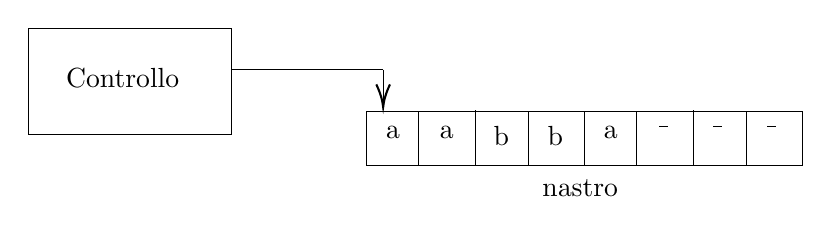
\begin{tikzpicture}[x=0.75pt,y=0.75pt,yscale=-1,xscale=1]
%uncomment if require: \path (0,300); %set diagram left start at 0, and has
%height of 300

%Shape: Rectangle [id:dp9416987304067759] 
\draw   (100,89) -- (198,89) -- (198,140) -- (100,140) -- cycle ;
%Shape: Rectangle [id:dp3803387153024198] 
\draw   (263,129) -- (368,129) -- (368,155) -- (263,155) -- cycle ;
%Straight Lines [id:da7053902512087236] 
\draw    (288,129) -- (288,155) ;
%Straight Lines [id:da5656119026072681] 
\draw    (341,129) -- (341,143) -- (341,155) ;
%Straight Lines [id:da6739796655004393] 
\draw    (315.5,128.5) -- (315.5,155.5) ;
%Straight Lines [id:da34292098732116805] 
\draw    (198,109) -- (271,109) ;
%Straight Lines [id:da9542933537032088] 
\draw    (271,109) -- (271,125) ; \draw [shift={(271,127)}, rotate = 270]
[color={rgb, 255:red, 0; green, 0; blue, 0 }  ][line width=0.75]
(10.93,-3.29) .. controls (6.95,-1.4) and (3.31,-0.3) .. (0,0) .. controls
(3.31,0.3) and (6.95,1.4) .. (10.93,3.29)   ;
%Shape: Rectangle [id:dp5825598898008435] 
\draw   (368,129) -- (473,129) -- (473,155) -- (368,155) -- cycle ;
%Straight Lines [id:da35919750793452043] 
\draw    (393,129) -- (393,155) ;
%Straight Lines [id:da26276249325561674] 
\draw    (446,129) -- (446,143) -- (446,155) ;
%Straight Lines [id:da10712862194666761] 
\draw    (420.5,128.5) -- (420.5,155.5) ;

% Text Node
\draw (117,107) node [anchor=north west][inner sep=0.75pt]   [align=left]
{Controllo};
% Text Node
\draw (271,135) node [anchor=north west][inner sep=0.75pt]   [align=left] {a};
% Text Node
\draw (297,135) node [anchor=north west][inner sep=0.75pt]   [align=left] {a};
% Text Node
\draw (323,135) node [anchor=north west][inner sep=0.75pt]   [align=left] {b};
% Text Node
\draw (349,135) node [anchor=north west][inner sep=0.75pt]   [align=left] {b};
% Text Node
\draw (346.5,160.5) node [anchor=north west][inner sep=0.75pt]   [align=left]
{nastro};
% Text Node
\draw (376,135) node [anchor=north west][inner sep=0.75pt]   [align=left] {a};
% Text Node
\draw (402,135) node [anchor=north west][inner sep=0.75pt]   [align=left] {\_};
% Text Node
\draw (428,135) node [anchor=north west][inner sep=0.75pt]   [align=left] {\_};
% Text Node
\draw (454,135) node [anchor=north west][inner sep=0.75pt]   [align=left] {\_};


\end{tikzpicture}

\end{center}

Il cuore della definizione di una macchina di Turing è la funzione di
transizione $\delta$ perché essa ci dice come la macchina effettua un passo. Per
una macchina di Turing, $\delta$ prende la forma

\begin{center}
    $Q \times \Gamma \rightarrow Q \times \Gamma \times \{L,R\}$
\end{center}

Cioè, quando la macchina occupa un certo stato q e la testina punta alla casella
del nastro contenente un simbolo a e se $\delta$(q, a) = (r, b, L), la macchina
scriverà il simbolo b al posto di a, passerà allo stato r e la testina si
sposterà verso sinistra dopo la scrittura.

--------------------------------------------------------------------------------------------------

\begin{center}
   \textcolor{red}{Definizione Formale di Macchina di Turing} 
\end{center}

Una \textbf{Macchina di Turing} è una 7-upla (Q, $\Sigma$, $\Gamma$, $\delta$,
$q_0$, $q_{accept}$, $q_{reject}$) dove Q, $\Sigma$ e $\Gamma$ sono tutti
insiemi finiti e:

\begin{enumerate}
    \item Q è l'insieme degli stati,
    \item $\Sigma$ è l'alfabeto di input non contenente il simbolo
    \textbf{blank},
    \item $\Gamma$ è l'alfabeto di nastro, con \textbf{blank} $\in \Gamma$ e
    $\Sigma \subseteq \Gamma$,
    \item $\delta$: $Q \times \Gamma \rightarrow Q \times \Gamma \times \{L,R\}$
    è la funzione di transizione,
    \item $q_0$ è lo stato iniziale,
    \item $q_{accept} \in Q$ è lo stato di accettazione,
    \item $q_{reject} \in Q$ è lo stato di rifiuto, con $q_{rej} \neq q_{acc}$.
\end{enumerate}

--------------------------------------------------------------------------------------------------

\subsection{Computazione e Configurazione di una Turing Machine}

Una macchina di Turing M = (Q, $\Sigma$, $\Gamma$, $\delta$, $q_0$,
$q_{accept}$, $q_{reject}$) \textbf{computa} nel seguente modo: inizialmente M
riceve il suo input $w_1w_2...w_n \in \Sigma^*$ sulle n celle più a sinistra del
nastro, mentre il resto del nastro contiene tutti simboli \textbf{blank}. La
testina parte dalla posizione più a sinistra del nastro. Si noti che $\Sigma$
non contiene il simbolo blank, così il primo di questi simboli segna la fine
dell'input.

La computazione finisce quando M entra in uno stato accettante o in uno di
rifiuto, altrimenti M entra in \textbf{loop}. Durante la computazione di una
macchina M si verificano cambiamenti dello stato corrente, del contenuto
corrente del nastro e della posizione corrente della testina. Un'impostazione di
questi tre elementi è chiamata \textbf{configurazione} della macchina di Turing.
Per uno stato q e due stringhe u, v sull'alfabeto $\Gamma$ del nastro, scriviamo
"u q v" per indicare la configurazione, dove:

\begin{enumerate}
    \item lo stato corrente è q,
    \item il contenuto corrente del nastro è u v,
    \item la posizione corrente della testina è il primo simbolo di v.
\end{enumerate}

Dopo l'ultimo simbolo di v, il nastro contiene solo simboli blank.

Formalizziamo ora come una macchina di Turing \textbf{computa}. Si dice che la
configurazione $C_1$ \textbf{produce} $C_2$ se la TM può passare da $C_1$ a
$C_2$ in un unico passo. Definiamo formalmente questa nozione nel seguente modo.

Supponiamo di avere a, b e c $\in \Gamma$, così come u e v $\in \Gamma^*$ e gli
stati $q_i e q_j$.

In tal caso "u a $q_1$ b v" e "u $q_j$ a c v" sono due configurazioni. Diciamo
che

\begin{center}
    \underline{u a $q_1$ b v} \textbf{produce} \underline{u $q_j$ a c v}
\end{center}

se nella funzione di transizione $\delta$($q_i$, b) = ($q_j$, c, L). Questo nel
caso in cui la macchina di Turing effettua uno spostamento verso sinistra.

\subsection{Linguaggi Turing-Riconoscibili e Turing-Decidibili}

L'insieme di stringhe che M accetta rappresenta il \textbf{linguaggio di M}, o
il \textbf{linguaggio riconosciuto da M}, denotato come L(M).

--------------------------------------------------------------------------------------------------

\begin{center}
    \textcolor{red}{Definizione}
\end{center}

Un linguaggio si dice \textbf{Turing-riconoscibile} se esiste una macchina di
Turing che lo riconosce.

--------------------------------------------------------------------------------------------------

Quando attiviamo una TM su un input, tre risultati sono possibili. La macchina
può:

\begin{enumerate}
    \item accettare,
    \item rifiutare,
    \item andare in loop.
\end{enumerate}

A volte distinguere una macchina che è entrata in un loop da una che sta
semplicemente impiegando tanto tempo risulta difficile. Per questo si
preferiscono macchine di Turing che che si fermano su ogni singolo input, ovvero
che non vanno mai in loop. 

Una tale macchina viene chiamata \textbf{decisore} perché in ogni caso prende
una decisione, sia essa di accettare o rifiutare l'input. Diciamo che un
decisore \textbf{decide} un certo linguaggio se riconosce tale linguaggio.

--------------------------------------------------------------------------------------------------

\begin{center}
    \textcolor{red}{Definizione}
\end{center}

Un linguaggio si dice \textbf{Turing-decidibile} o semplicemente
\textbf{decidibile} se esiste una TM che lo decide.

--------------------------------------------------------------------------------------------------

\subsection{Varianti di Macchine di Turing}

Esistono molte definizioni alternative di macchine di Turing, comprese le
versioni multinastro o non-deterministiche. Esse sono dette \textbf{varianti}
del modello macchina di Turing. Il modello originale e le sue varianti hanno
tutte \textbf{lo stesso potere computazionale}, ovvero riconoscono la stessa
classe di linguaggi.

In questa sezione descriviamo alcune varianti e le relative prove di equivalenza
in termini di potenzialità.

\noindent Un primo esempio può essere una variante in cui, ad ogni passo
computazionale, la macchina può non dover muovere la testina, modificando così
la funzione di transizione da

\begin{center}
    $\delta: Q \times \Gamma \rightarrow Q \times \Gamma \times \{L, R\}$

    in

    $\delta: Q \times \Gamma \rightarrow Q \times \Gamma \times \{L, R, S\}$
\end{center}

Questa caratteristica non permette in nessuno modo alle macchine di Turing
create in questo modo di riconoscere nuovi linguaggi.

Questo perché possiamo dividere in due transizioni (prima muovo la testina verso
sinistra, poi la riporto a destra qualsiasi simbolo io legga e senza scrivere
nulla) la transizione in cui la testina deve rimanere ferma.

Questo esempio contiene la chiave per poter mostrare l'equivalenza di varianti
di TM. Per dimostrare che due macchine sono equivalenti, abbiamo bisogno di
dimostrare che \textbf{ognuno dei due modelli può simulare l'altro}.

\subsubsection{Macchina di Turing Multinastro}

Una macchina di Turing multinastro è essenzialmente una generalizzazione della
macchina di Turing a nastro singolo. Ogni nastro ha la sua testina per la
lettura/scrittura.

Inizialmente l'input si trova sul nastro 1, mentre gli altri nastri sono vuoti.
La funzione di transizione viene modificata per consentire la scrittura, la
lettura e lo spostamento della testina contemporaneamente su alcuni o tutti i
nastri, formalmente:

\begin{center}
    $\delta: Q \times \Gamma^k \rightarrow Q \times \Gamma^k \times \{L, R,
    S\}^k$
\end{center}

dove k è il numero di nastri. L'espressione

\begin{center}
    $\delta(q_i, a_1, ..., a_k) = (q_j, b_1, ..., b_k, L, R, ..., L)$ 
\end{center}

significa che, se la macchina si trova nello stato $q_i$ e le testine da 1 a k
leggono i simboli da $a_1$ a $a_k$, la macchina va nello stato $q_j$, scrive i
simboli da $b_1$ a $b_k$ e muove ogni testina a sinistra o a destra, o la fa
restare ferma, come specificato.

\newpage

--------------------------------------------------------------------------------------------------

\begin{center}
    \textcolor{red}{Teorema}
\end{center}

Per ogni macchina di Turing multinastro esiste una macchina di Turing a nastro
singolo equivalente.

--------------------------------------------------------------------------------------------------

Dimostriamo ora che questa variante di TM non aggiunge potenza alla TM base, per
farlo ricordiamo che due macchine sono equivalenti se riconoscono lo stesso
linguaggio.

\textbf{DIMOSTRAZIONE}. Mostriamo come convertire una macchina di Turing
multinastro M in una TM S equivalente a nastro singolo. L'idea chiave è di
mostrare come \textbf{simulare} M con S.

Supponiamo che M abbia k nastri, allora S simula l'effetto di k nastri
memorizzando le loro informazioni sul suo singolo nastro. Essa utilizza un nuovo
simbolo "\#" come delimitatore per separare i contenuti dei diversi nastri.
Invece, per tenere traccia delle posizioni delle testine, S marca il simbolo in
cui dovrebbe essere posizionata la testina per tutti i contenuti dei "nastri
virtuali".

\subsubsection{Macchina di Turing non Deterministica}

Una macchina di Turing non deterministica è definita come ci si aspetta. In ogni
passo della computazione la macchina può procedere effettuando varie scelte. Per
questo la funzione di transizione va modificata e risulta essere del tipo:

\begin{center}
    $\delta: Q \times \Gamma \rightarrow \mathcal{P}(Q \times \Gamma \times \{L,
    R\})$
\end{center}

--------------------------------------------------------------------------------------------------

\begin{center}
    \textcolor{red}{Teorema}
\end{center}

Per ogni macchina di Turing non deterministica esiste una macchina di Turing
deterministica equivalente.

--------------------------------------------------------------------------------------------------

\textbf{DIMOSTRAZIONE.}  La TM D deterministica che simula la TM N non
deterministica ha tre nastri. D utilizza questi tre nastri in maniera
particolare.

\begin{enumerate}
    \item Il primo nastro contiene sempre la stringa di input e non viene mai
    modificato
    \item Il secondo nastro mantiene una copia del nastro di N corrispondente a
    qualche diramazione non deterministica
    \item Il terzo nastro tiene traccia della posizione di D nell'albero delle
    computazioni di N
\end{enumerate}

\subsubsection{Enumeratori}

\textcolor{red}{RICORDA DI FINIRE QUESTA PARTE}

\section{Decidibilità}

In questo capitolo cominciamo ad investigare la potenza degli algoritmi nella
risoluzione di problemi.

Dimostreremo che alcuni problemi possono essere risolti in maniera algoritmica
ed altri no. Il nostro obiettivo è esplorare i limiti della risolvibilità
algoritmica dei problemi. 

\subsection{Linguaggi Decidibili}




\end{document}